
\section*{\textbf{\underline{Abstract}}}
Predicting the assembly processes of competitive communities is nontrivial and often requires estimating interspecific pairwise effects. However, interaction-explicit approaches become increasingly difficult as community size increases. Demographic rates measured in single-species cultures may provide a simpler basis for prediction than interaction-explicit approaches, but the conditions under which monoculture-derived parameters scale to multispecies communities remain unclear. Here, we use experimental communities of phenotypically distinguishable strains of brewer's yeast (\textit{Saccharomyces cerevisiae}) to test whether demographic parameters derived from monoculture growth experiments can predict multi-strain community outcomes across nutrient environments. We find that simulations parameterized by strain-specific estimates of finite rate of increase (R) and carrying capacity (K) closely match empirical communities under low nutrient conditions, but matched empirical communities less closely under high-nutrient conditions. Empirical communities also deviated more strongly from equal starting composition in high-nutrient than low-nutrient conditions. Together, our results show that single-species growth parameters can provide useful predictions of community assembly, but that their predictive value depends on environmental context. 


% TAD: I would hesitate to use the 'low' dimension argument. It will likely rub many theory people the wrong way, because it's not actually lower in dimension, right? To predict community assembly, you need the alpha matrix and those demographic parameters, and Chesson would say you just need the alpha matrix. So a shit ton of research has been focused on that alpha matrix, and you're coming in just like "yolo, assume diffuse competition, or like equivalent competition, and it's the demographic rates we care about". Maybe fine, maybe tough sell. Don't send it to Mike Fowler, Ellner, Tulja, or many other people.

%GF: I've tried to remove most of the references to "low-dimsension," but I do think in principle the gist is the same. As it stands it is kind of competing with Chesson's view in a really simple system, and even then it only works some of the time. I've tried to rewrite the intro and parts of the discussion to engage with this more, though maybe still not enough. 


% TAD (after full read through). It's not bad. There is some definite language changes that need to happen, and the 'low dimension' stuff is odd. Some narrative points could be sharpened, most notably in the first paragraph of the discussion, which just read like results to me with one sentence at the end for interpretation. It's super citation light for you, and it's one where it feels like there should be a lot of citations. Are there no good papers to cite from the HillResLambers Annual Review paper? No mention of current theoretical paradigms of community assembly is also a bit odd. Not even as much discussion of neutral theory as I would have expected, but it creeps in there (and then you poop on it by spending a massively long discussoin paragraph talking about pigments). It's probably good for dissertation with some clarity edits and fixes (maybe more some cites added in), but I wouldn't submit this until it gets some further development. 

\clearpage


%-----------------------------
\section*{\textbf{\underline{Introduction}}}
\paragraph*{} Understanding and predicting how biological communities assemble is necessary to understand how biodiversity is structured across space and time. The predictability of assembly outcomes has been a major research focus in classical community ecology  \parencite{diamond1975assembly,drake1990mechanics, keddy1992assembly, weiher2001ecological,chase2003community, tilman2004niche}. Traditional community assembly paradigms emphasize the importance of abiotic and biotic filters on determining how regional species pools translate into local communities  \parencite{weiher2011advances, hillerislambers2012rethinking}. However, at the site level assembly outcomes are influenced by both demographic stochasticity and species-level niche and competitive differences \parencite{tilman2004niche, macdougall2008climatic, martorell2014testing, zhou2017stochastic}, and untangling the relative importance of stochastic and deterministic processes is difficult, though increasingly possible through advanced statistical approaches \parencite{Maynard2020}.

% TAD: ....and I'm stopping here with super detailed comments. I'll still make some line suggestions, but the sentence above talks about separating roles but doesn't define what the 'roles' are, so it reads bad. "these experiments" below without referencing what experiments you refer to (i.e. experiments that estimate pairwise interaction coefficients, or at least just pairwise competition experiments, I think is what you mean?

\paragraph*{} Modern coexistence theory emphasizes members of coexistent communities should be able to invade equilibrial communities when rare  \parencite{chesson2000mechanisms, hillerislambers2012rethinking}. Demographic studies that characterize how the growth rates of one species depend on the frequency of competitors can be used to predict both coexistence and assembly outcomes \parencite{wills1997strong, hille2002density, harpole2007frequency}. However, pairwise competition experiments are difficult, and become increasingly intractable as community size increases \parencite{maurer1999untangling}. Additionally, predictions based on pairwise interactions may fail when multispecies outcomes depend on emergent higher order effects or environmental context dependence \parencite{chesson2018updates,lee2023resource, miller2025multispecies}. Alternative approaches look to predict community outcomes from lower dimensional data, including community abundance timeseries \parencite{carrara2015inferring} or single species experiments \parencite{nestor2023interactions}. At one extreme, neutral theory, which ignores species-level differences and simulates community composition through stochastic processes, while inherently simplifying can recapitulate patterns observed in some empirical communities \parencite{Hubbell2001, woodcock2007neutral, oficteru2010combined}. Between fully neutral models and interaction-explicit approaches are models that retain measurable differences among species, such as growth rate or carrying capacity, while simplifying the structure of interspecific interactions between species. 

\paragraph*{} Single species vital rates are one possible source of simplified demographic information, and may help predict community outcomes \parencite{ram2019predicting, nestor2023interactions}. However, the scaling from population to community outcomes is not always straightforward \parencite{khristich2025empirical}. Demographic rates derived from monoculture describe how the vital processes of a given species scale with its own density. In communities strongly structured by antagonistic interactions, differences between intra- and interspecific competitive effects may strongly influence assembly outcomes \parencite{hillerislambers2012rethinking,barabas2016effect, chesson2018updates}. Failing to account for these differences may therefore limit the ability of single-species vital rates to predict community outcomes. In some systems, functional traits or phylogenetic distances can help approximate these pairwise effects \parencite{cadotte2013ecology, e2023phylogenetic}. However, in communities where species are weakly structured by direct interactions, or where species contribute similarly to shared density limitation, single-species vital rates may be sufficient to predict community-level outcomes. 

\paragraph*{}
The utility of single-strain vital rates may also depend on environmental context. The strength and mechanisms governing species interactions can vary across environments \parencite{van2022small}, potentially changing whether monoculture dynamics capture the processes driving final community composition. Nutrient availability may be especially important because it can alter both the densities that populations reach and the relative importance of different competitive mechanisms, including shared resource limitation, metabolite accumulation, and interference competition \parencite{salvado2011quantifying, albergaria2016dominance}. As a result, both community assembly outcomes and the predictability of those outcomes may be dependent on resource availability.

% TAD: is it really about the ability to predict outcomes? I like the env angle as saying "community assembly outcomes may be dependent on resource availability, unlike what MCT or neutral theory would predict" 

%GF: Fair; I was trying to ply the prediction angle to tie in to the single=species growthrates part, but it is more about the assembly outcomes themselves. I do think that's in opposition to neutral theory, but would argue that hardcore MCT folks would say that MCT could still work, but the alpha-values underlying it change as a function of the enviornment (so you have to check them). 

\paragraph*{} Microbial communities are especially useful for testing questions about community assembly because they are highly replicable and can be assembled under controlled environmental conditions \parencite{nemergut2013patterns}. These features make it possible to manipulate both community composition and environmental context while directly measuring the outcomes of assembly. By experimentally standardizing the species pool, initial abundances, and abiotic environment, microbial systems allow local assembly processes to be isolated from broader biotic and abiotic filtering effects observed in natural systems \parencite{weiher2011advances}. Phenotypically distinguishable strains of \textit{Saccharomyces cerevisiae} with a shared genetic background provide an especially controlled system for testing community assembly dynamics \parencite{mitchell2015versatile}. By reducing many of the taxonomic, phylogenetic, and physiological differences that complicate prediction in natural communities, this system provides a conservative test of whether monoculture growth parameters can predict community assembly under different environmental conditions. 

% Statement of research questions and hypotheses. 
\paragraph*{}
Here, we use experimental communities of phenotypically distinguishable strains of brewer's yeast (\textit{Saccharomyces cerevisiae}) to test whether single-species vital rates scale to community-level outcomes. By comparing experimental communities to those simulated from single-species vital rates, we test whether nutrient availability alters the predictability and assembly of multi-species communities. We show that nutrient environment has no detectable effect on the finite rate of increase, but large effects on the carrying capacity for a given strain in monoculture. We further find that multistrain communities are well predicted by simulation models parameterized by single-species vital rates in low nutrient environments, but not in high nutrient environments. Together our results highlight the environmental-dependence of community assembly outcomes, even in highly simplified experimental communities.


\section*{\textbf{\underline{Methods}}}
\paragraph*{Yeast System}\mbox{}\\
We used a series of yeast strains with biosynthetic pigment pathways assembled on episomal VEGAS (Versatile genetic assembly system) assembly vectors created using a yeast Golden Gate approach, detailed in  \textcite{mitchell2015versatile}. The result is a series of yeast strains with identical genetic backgrounds, but containing cytosolic shuttle plasmids that encode biosynthetic pigment pathways, along with selectable markers (KanMX and URA3), and as such are visually distinct due to pigment production. Three strains include combinatorial 3 or 4-gene beta carotene pathways (hereafter the red, orange, and yellow strains), while a fourth contains the pathway to synthesize violacein (hereafter the black strain). 

\paragraph*{Monoculture Growth Curves}\mbox{}\\
We used liquid cultures to estimate strain-specific vital rates. Liquid cultures of each strain were diluted 1,000 fold in full-strength media (25g/L Difco\textsuperscript{TM} YPD broth powder, Becton, Dickinson, and Company), and 20$\mu L$ was then used to inoculate 180$\mu L$ sterile cultures within wells of a 96-well plate. In high-nutrient treatments, sterile cultures were made of YPD solution. In low-nutrient treatments sterile cultures were prepared with DI water, making the final working concentration of 2.5g YPD per liter (10\% of laboratory standard concentrations). Culture plates were incubated for 20 hours at 30 degrees Celsius inside a temperature-controlled spectrophotometer. Every ten minutes cultures were shaken for 5 seconds prior to recording optical density at 600nm. Split across 3 trials, we measured 12 replicate growth curves for each strain at low-nutrient concentrations, and 8 replicate curves for each strain at high-nutrient conditions. One growth curve trial (4 replicates) of orange at low density showed anomalously high absorbance values, and was discarded from the analysis. 

% TAD: I'd probably talk about how we got the standard curves (someone may be critical of estimating abundance from colonies?) 
%GF: I can add in the standard curve part (it's basically growing colonies up to carrying capacity, counting density under a scope, and then doing serial dilutions + measuring their absorbance). We're not lookign at absolute density in our multispecies communtieis at all right now though; only relative densities. Biggest sketch part is that we're assuming there aren't enough pigment differences between colors, so we're just applying the white curve to all of them. 

\paragraph*{}
We used nutrient-specific linear standard curves generated from wild-type liquid culture, and applied them across pigment strains under the assumption that pigment effects on OD600 in liquid culture were small relative to differences in cell abundance. Visible pigment differences developed slowly relative to the timescale of our growth curve assay, becoming most distinct after several days of colony growth on agar plates. We fit the resulting abundances to a discrete logistic growth model under a Bayesian hierarchical framework in STAN \parencite{carpenter2017stan} as implemented through the package \textit{cmdstanr} \parencite{gabry2021cmdstanr}, such that 
\begin{equation}
    N_{n,t+1}=N_{n,t}+R_nN_{n,t}\left(1-\frac{N_{n,t}}{K_n}\right)
\end{equation}
 The finite rate of increase (R) and carrying capacity (K) were estimated separately for each strain-by-nutrient combination; each timestep of our discrete model represented a 10 minute interval between OD600 measurements. Replicate trajectories were allowed to vary in R around their corresponding strain-by-nutrient mean, with a single replicate-level variance parameter shared across all groups. Observation error was modeled with a shared lognormal error term, and weakly informative priors were placed on log-transformed vital-rate parameters and variances. Models were fit using four MCMC chains with 1000 timesteps following a 1000-timestep burn-in period. Models were checked for convergence by analyzing ESS and $\hat{R}$ for each parameter estimate, as well as through posterior predictive visualizations. 
%Priors are quite broad (log_R_group ~ normal(log(1), 1); log_K_group ~ normal(log(3), 2);


\paragraph*{Polyculture communities}\mbox{}\\
We created multi-strain polyculture communities by inoculating sterile media with different combinations of single-species liquid cultures at the same relative abundance across a community. To ensure initial abundances were the same across strains, cell density estimates were recorded via hemocytometer for each single-species culture. We adjusted initial inoculation amounts based on measured standard densities. For each monoculture, 1mL sterile cultures were inoculated with 100$\mu$L of the least abundant culture, or the equivalent amount of more abundant standards. Polycultures were inoculated with an equivalent total amount of yeast, split evenly between present strains so that all strains begin at the same relative and total abundances. 

Communities were vortexed, and 200$\mu$L samples were added to wells of a 96-well plate, and passaged in an incubated spectrophotometer for 24 hours. To measure relative abundance of strains within each community, communities were subsampled and diluted to either 1:1000 (high-nutrient) or 1:100 (low-nutrient), and then used to inoculate two spread plates per community on agar media (25g/L YPD, Kanamycin 50mg/L). We created 8 community types in all; four single-strain communities (yellow, red, orange, and black), two two-strain communities (yellow-black and yellow-red), one three-strain community (yellow-red-black), and one four-strain community (yellow-orange-red-black). We created eight replicates of each community per nutrient treatment; after incubation each community was sampled twice to improve estimates of relative abundance and plate-to-plate variation, for a total of 256 community samples. Spread plates were incubated at 30 degrees Celsius for 48 hours, after which pigments were allowed to saturate by holding the colonies at approximately 2 degrees Celsius for two weeks. After this period plates were photographed and the number of colonies of each strain were counted from photographs. 43 samples were discarded either due to contamination or low overall abundance (<5 colonies), leaving a total of 213 communities (Table \ref{tab:contamination_outcomes}).   

Strains were maintained on selective agar (Kanamycin 50mg/L) prior to experiments, but antibiotic selection was not maintained during the 20-hour liquid growth and polyculture assays. Although experimental communities were inoculated only with colored strains, a minority of colonies did not express visible phenotypes and could instead appear wild-type appearing (mean = 15.2\% across strain-nutrient combinations). Because loss or reduced expression of pigment pathways could produce wild-type-appearing colonies, and because these colonies in multispecies communities could originate from any strain present, we used a Bayesian hidden-state model informed by monoculture expression rates and observed phenotype counts to estimate underlying strain relative abundances in each final community. Details of the model structure and uncertainty around relative abundance estimates are presented in the supplement.

\paragraph*{Community Simulations}\mbox{}\\
\paragraph{} To test whether monoculture vital rates were sufficient to predict community composition, we simulated each multistrain community using strain-by-nutrient posterior estimates of R and K.  We began simulations at the mean initial starting abundance across all community replicates, and then simulated 144 timesteps (24 hours of development) of a multispecies discrete logistic growth model, using the equation 
\begin{equation}
    N_{n,t+1}=N_{n,t}+\max\left[
    R_nN_{n,t}\left(1-\frac{\sum_i N_{i,t}}{K_n}\right), 0
    \right].
\end{equation}. 
For each focal strain (n), density dependence was determined by total community abundance, ($\sum_i N_{i,t}$), scaled by the focal strain's monoculture carrying capacity, ($K_n$). This formulation assumes equivalent intra- and interspecific competitive effects among all strains, corresponding in a Lotka-Volterra framework \parencite{volterra1928variations, macarthur1967limiting} to a competition matrix in which all interaction coefficients are equal to 1. Because our experiment was conducted over a short timescale during which cell division was expected to dominate changes in abundance over mortality, we constrained population size to increase monotonically. We therefore set population growth rate, ($R_nN_{n,t}(1-\sum_i N_{i,t}/K_n)$), to zero whenever it would otherwise be negative. Therefore final relative abundances within a community are determined both the finite rate of increase (R) and carrying capacities (K) of strains within the community. We simulated 1000 iterations of each community using sampled R and K values for each strain from fit posterior distributions, and the distribution of simulated community outcomes was compared to those observed empirically. Wilson's score intervals were used to compare colony counts across plates within a given treatment. Relative abundances were compared using 95\% credible intervals and pairwise contrasts across strains. Throughout the Results, we interpreted pairwise differences as supported when the 95\% credible interval for a contrast did not overlap zero, and interpreted observed and simulated outcomes as different when their 95\% credible intervals did not overlap.

% TAD: be explicit about the assumption of equal competitive pressure above. That's basically what you're doing by letting all species contribute to the carrying capacity, right? All entries of the alpha matrix are 1. 
%GF: Added


%----------
\section*{\textbf{\underline{Results}}}
\paragraph*{Monoculture growth parameters differed among strains and nutrient environments}\mbox{}\\
Strain-specific carrying capacity differed strongly across nutrient environments (Figure \ref{fig:VitalRates}). Across all strains, high-nutrient carrying capacities were approximately an order of magnitude larger than low-nutrient carrying capacities. Despite a large shift in absolute carrying capacity, the relative ranking of strains was broadly consistent across nutrient treatments. The black strain had the lowest estimated carrying capacity in both low- and high-nutrient environments, while red and orange had the highest estimated carrying capacities. Yellow and wild-type strains were intermediate, with overlapping 95\% credible intervals in both nutrient environments.

In contrast, finite rate of increase varied more among strains than between nutrient environments (Figure \ref{fig:VitalRates}). For each strain, 95\% credible intervals for (R) overlapped between low- and high-nutrient treatments. Black, yellow, and wild-type strains generally had higher estimated (R) values than red and orange, although several strain-level intervals overlapped. Posterior estimates also suggested a negative relationship between R and K across strains (see supplement Figure \ref{fig:Sup_RvsKscaling}). Together, these results indicate that nutrient availability strongly altered monoculture carrying capacity while having comparatively little effect on estimated finite rate of increase.

\paragraph*{Empirical communities deviated from equal starting composition}\mbox{}\\
Although all polyculture communities were inoculated at equal starting relative abundances, final strain composition was often nonequivalent (Figure \ref{fig:CommunityBarcharts}). These deviations were most pronounced under high-nutrient conditions. In high-nutrient environments, the yellow strain increased in relative abundance across all community types in which it was present; in each case, the 95\% credible interval for change in relative abundance was entirely above zero. Black, red, and orange strains were generally similar in final relative abundance, with 95\% credible intervals for most pairwise contrasts overlapping zero, although black slightly exceeded red in the four-strain community (Figure \ref{fig:Contrasts}). In low-nutrient environments, final community composition was closer to equal relative abundance across strains. The black strain tended to achieve slightly higher final abundance than the other strains across community types (95\% credible intervals of relative abundance pairwise contrasts were slightly above, but not overlapping 0), while most other pairwise differences were small. 



\paragraph*{Monoculture-parameterized simulations predicted low-nutrient communities better than high-nutrient communities}\mbox{}\\
Simulated community outcomes generally matched empirical community composition, particularly in the low-nutrient treatment (Figure \ref{fig:Contrasts}). In low-nutrient communities, 95\% credible intervals for observed and simulated pairwise contrasts overlapped in all cases except the red-orange contrast in the four-strain community, where red was more abundant and orange less abundant than predicted (Figure \ref{fig:Contrasts}).

Observed and simulated communities diverged more strongly under high-nutrient conditions, especially in more diverse communities. 95\% credible intervals of simulated and observed outcomes overlapped in both high nutrient two-strain communities. However, in high-nutrient three- and four-strain communities empirical estimates of black relative abundance were lower than simulated estimates, with non-overlapping 95\% credible intervals. Across comparisons, high-nutrient communities tended to show larger-magnitude deviations from both equal starting composition and monoculture-based predictions. 

% TAD you use language to suggest a statistical test was performed (showed greater diverengence, was lower, etc.), but where are the statistics? 
%GF: My bad; it's 95\% credible intervals all the way down. Tried to make this more specific in these two paragraphs, added a sentence trying to be really specific about what comparisons I'm using to say what in the last sentence of the methods. 


%-----------------------------
\section*{\textbf{\underline{Discussion}}}
%2: Competitive interactions near carrying capacity may be very different across treatments; that's what's cool about the fact only one nutrient environment is predictable. 
\paragraph{} Our results demonstrate that nutrient availability can alter both community assembly outcomes and the predictability of those outcomes, even in highly simplified experimental communities. The difference between low- and high-nutrient environments may reflect a shift in the density-dependent processes structuring these communities. Nutrient availability had no detectable effect on finite rate of increase, but strongly altered carrying capacity, suggesting that the two nutrient treatments differed primarily in the densities that populations could reach rather than in their early per-capita growth. In resource-poor, low-density environments, exploitation competition over shared nutrient resources, such as dextrose and peptides, may be more influential in shaping competitive outcomes \parencite{hoek2016resource}. In contrast, at high resource levels, interference competition (in the form of metabolite or toxin production \parencite{greig2008density}, cell-cell signaling \parencite{honigberg2011cell}, or other mechanisms \parencite{perez2017ecological}) may be more important for determining pairwise and ultimately community-level outcomes. Nutrient-dependent changes in density dependence may therefore help explain why single-strain growth parameters predicted community outcomes more accurately in low-nutrient than high-nutrient environments, emphasizing how the environmental contexts of competitive outcomes may be key to predicting community assembly. 

%3: Model interpretation. Monoculture vital rates can provide useful, but their predictive success is conditional on environment.
\paragraph{} Single-species vital rates scaled to community-level outcomes in some strain-by-nutrient combinations, but not others. Our simulation framework provides a simplified expectation for community assembly based on monoculture growth parameters \parencite{ram2019predicting, nestor2023interactions}. In this sense, the model occupies an intermediate position between neutral models, which assume species equivalence \parencite{Hubbell2001}, and interaction-explicit coexistence models \parencite{chesson2000mechanisms, chesson2018updates}.  The close agreement between simulated and observed communities in low-nutrient environments suggests that these parameters captured much of the relevant density-dependent structure in that treatment. In contrast, disagreement in high-nutrient environments indicates that monoculture growth parameters were insufficient to explain community composition under those conditions. This environment-dependent mismatch is consistent with nutrient conditions altering the interaction processes that shape community composition, reinforcing the view that niche-based and neutral processes may vary in relative importance across environmental contexts \parencite{weiher2011advances}.  

%4: Strain-specific explanation and limitations
\paragraph{} Most of the mismatch between simulated and empirical communities was associated with the black strain reaching lower relative abundance than predicted in high-nutrient environments. Based on monoculture growth parameters, simulations predicted that the black strain would outperform red and orange strains and reach similar final abundance to yellow in high-nutrient communities. Instead, black had lower relative abundance than yellow across multistrain communities and showed little or no advantage over red or orange. One possible explanation is that the engineered pigment pathways differed in their physiological costs. In our system, red, orange, and yellow pigmentation is produced through beta-carotene-related pathways, whereas black pigmentation is produced through a violacein pathway \parencite{mitchell2015versatile}. These pathways likely differ in biosynthetic demands (for example, beta-carotenes are hydrocarbons \parencite{maoka2020carotenoids} while violacein is nitrogenous \parencite{choi2015violacein}), and those differences could alter competitive performance in ways not captured by monoculture growth parameters. The black strain also had the highest estimated single-strain finite rate of increase, suggesting that growth-competition tradeoffs could contribute to its lower-than-expected performance in high-nutrient communities \parencite{kurihara1990trade}. However, our experiment cannot distinguish among pigment-production costs, plasmid instability, metabolite sensitivity, or other mechanisms. Black also produced wild-type-appearing colonies more often than the other pigment strains, suggesting that pigment-pathway instability or loss of visible phenotype may contribute additional uncertainty to its inferred 
abundance (Figure \ref{fig:FullModel_CommunityBarcharts}). However, as models of final strain abundances were informed by monoculture phenotype-expression rates, the observed differences between predicted and observed relative abundances in high-nutrient environments are unlikely to be caused by differential phenotype expression unless expression rates greatly differed between monoculture and mixed communities.

%5: Broader significance
\paragraph{}Together, our results show that single-species growth parameters can provide useful predictions of community assembly, but that their predictive value depends on environmental context. Our experiment used a deliberately simplified community composed of closely related yeast strains with a shared genetic background, yet prediction from vital rates alone remained imperfect. Monoculture-parameterized simulations predicted assembly in low-nutrient environments but not high-nutrient environments, suggesting that even minimal communities can exhibit context-dependent departures from models that simplify interaction structure. Community-level outcomes are difficult to predict, yet ecological processes such as stability, resilience, and ecosystem function depend on community structure \parencite{de2013predicting, tilman2014biodiversity}. Future work should identify how competitive mechanisms and density dependence vary across environmental gradients, and when additional interaction-specific parameters are necessary to predict community responses to environmental change.

\clearpage


\section*{\textbf{\underline{Figures}}}
\begin{figure}[h!]
  \begin{center}
    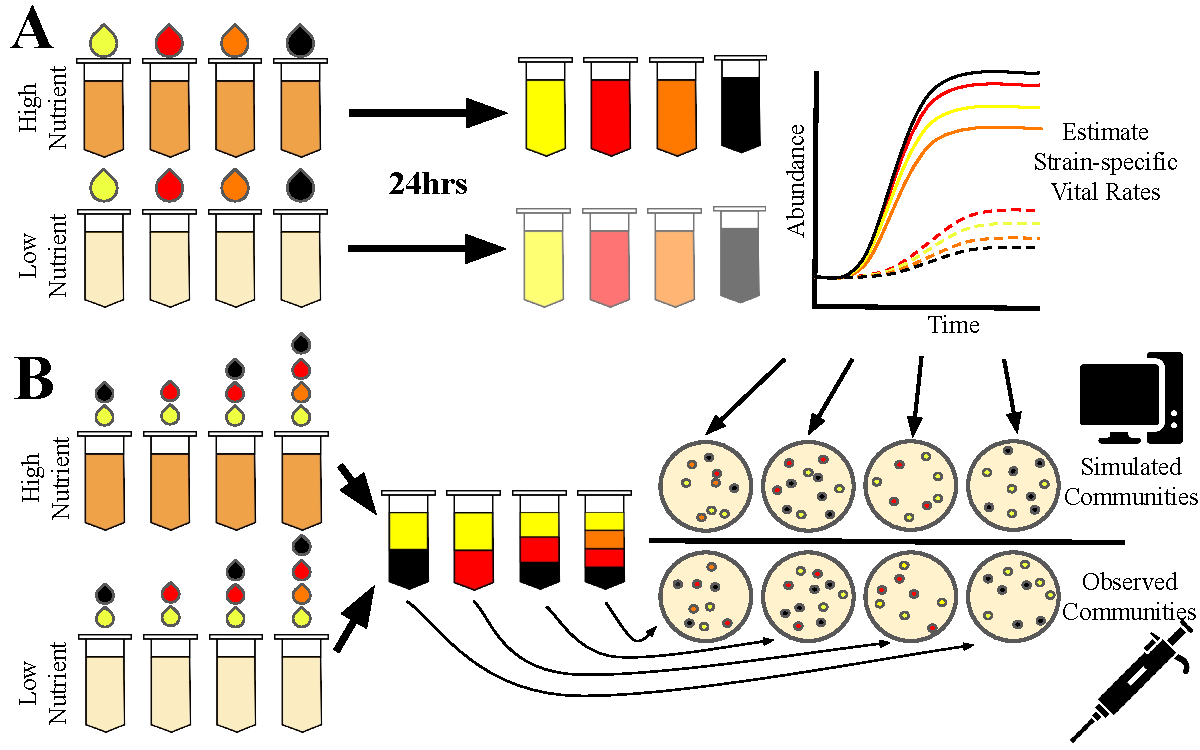
\includegraphics[width=\textwidth, alt={Conceptual workflow diagram with two panels. Panel A shows four yeast strains grown separately as monocultures in either high- or low-nutrient liquid media. After 24 hours, each culture reaches a different final abundance, illustrated by varying tube fill colors and accompanied by growth curves showing strain-specific population trajectories approaching carrying capacity. These measurements are used to estimate each strain's intrinsic growth rate and carrying capacity under both nutrient conditions. Panel B shows experimental communities assembled from equal starting abundances of multiple yeast strains and grown for 24 hours in the same two nutrient environments. Final mixed cultures are sampled by plating onto agar, where colonies of different colors represent different strains. The observed colony compositions are compared with communities simulated from the strain-specific growth parameters estimated in Panel A to evaluate whether single-strain growth dynamics predict multispecies community assembly.
}]{NutrientNeutrality/Figures/ConceptDraft.pdf}
    \caption[Conceptual overview of our experimental approach.]{Conceptual overview of the experimental approach. A) Sterile liquid monocultures were inoculated with each yeast strain and passaged in an incubated spectrophotometer, allowing populations to approach carrying capacity. These monocultures were used to estimate strain-specific carrying capacity (K) and finite rate of increase (R) in both low- and high-nutrient environments. B) Yeast communities were then inoculated with equal starting abundances of multiple strains and incubated for 24 hours under the same nutrient treatments. Final communities were subsampled by spread plating, and strain relative abundances were estimated from colony phenotypes. Comparing observed community composition with communities simulated from strain-specific vital rates allowed us to test whether multispecies community assembly can be predicted from single-strain growth dynamics.}
    \label{fig:conceptNutrient}
  \end{center}
\end{figure}

%Vital Rates as estimated by monoculture experiments
\begin{figure}[h!]
  \begin{center}
    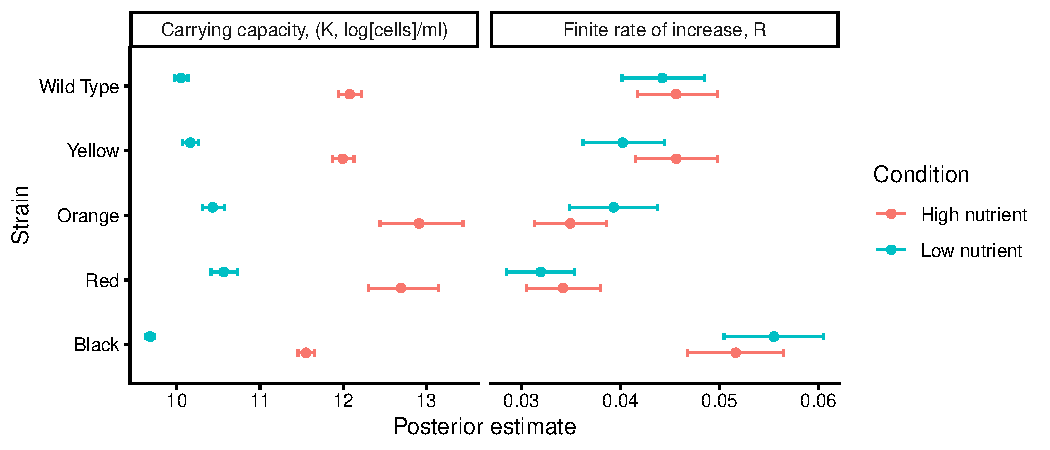
\includegraphics[width=\textwidth, alt={Plots visualizing strain-specific vital rates estimated from single-species liquid cultures}]{NutrientNeutrality/Figures/VitalEst.pdf}
    \caption[Strain-specific vital rates estimated from single-species liquid cultures.]{Strain-specific vital rates estimated from single-species liquid cultures. Points represent posterior mean estimates from the Bayesian logistic model, and horizontal lines represent 95\% credible intervals. Carrying capacity (\textit{K}, log scale) differed strongly between nutrient environments across all strains, with higher carrying capacities in the high-nutrient treatment. In contrast, finite rate of increase (\textit{R}) showed comparatively little sensitivity to nutrient environment. Strains also differed in their estimated vital rates, with red and orange strains generally exhibiting higher carrying capacities and lower R across nutrient environments.}
    \label{fig:VitalRates}
  \end{center}
\end{figure}

%Vital Rates as estimated by monoculture experiments
\begin{figure}[h!]
  \begin{center}
    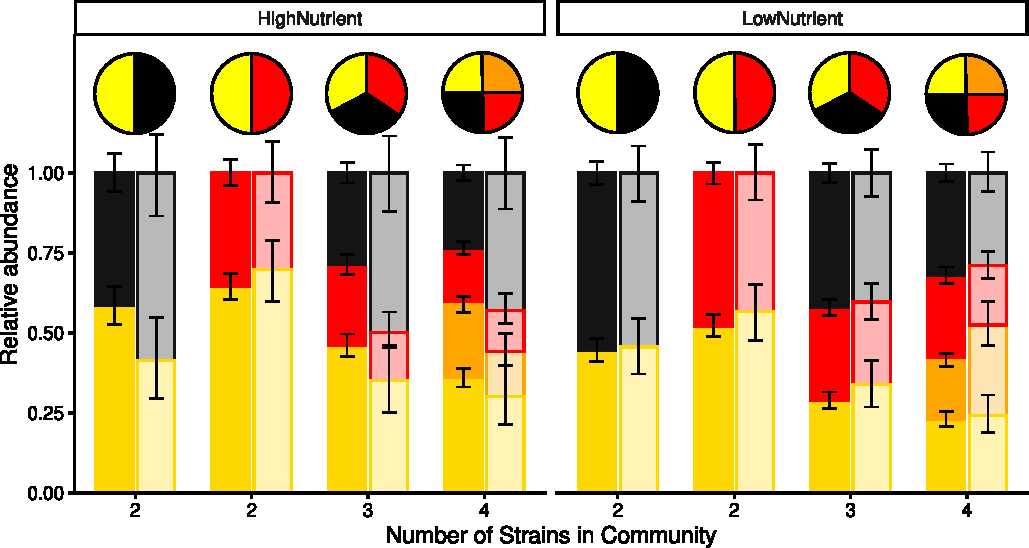
\includegraphics[width=\textwidth, alt={Stacked barcharts illustrating relative abundance of strains across community compositions and nutrient envrionment}]{NutrientNeutrality/Figures/ComparisonBarchart_icons.pdf}
    \caption[Relative abundance of strains across community compositions]{Modeled observed (opaque bars) and simulated (lighter bars) relative abundance of strains across community compositions; error bars represent 95\% credible intervals. In high-nutrient environments (left), the black strain exhibits lower relative abundance in experimental multistrain communities than predicted by models parameterized by monoculture vital rates. In contrast, in low-nutrient environments (right) experimental communities generally match those predicted by monoculture vital rates.}
    \label{fig:CommunityBarcharts}
  \end{center}
\end{figure}


%Final figure: comparing simulated community expectations to our empirical data   
\begin{figure}[h!]
  \begin{center}
    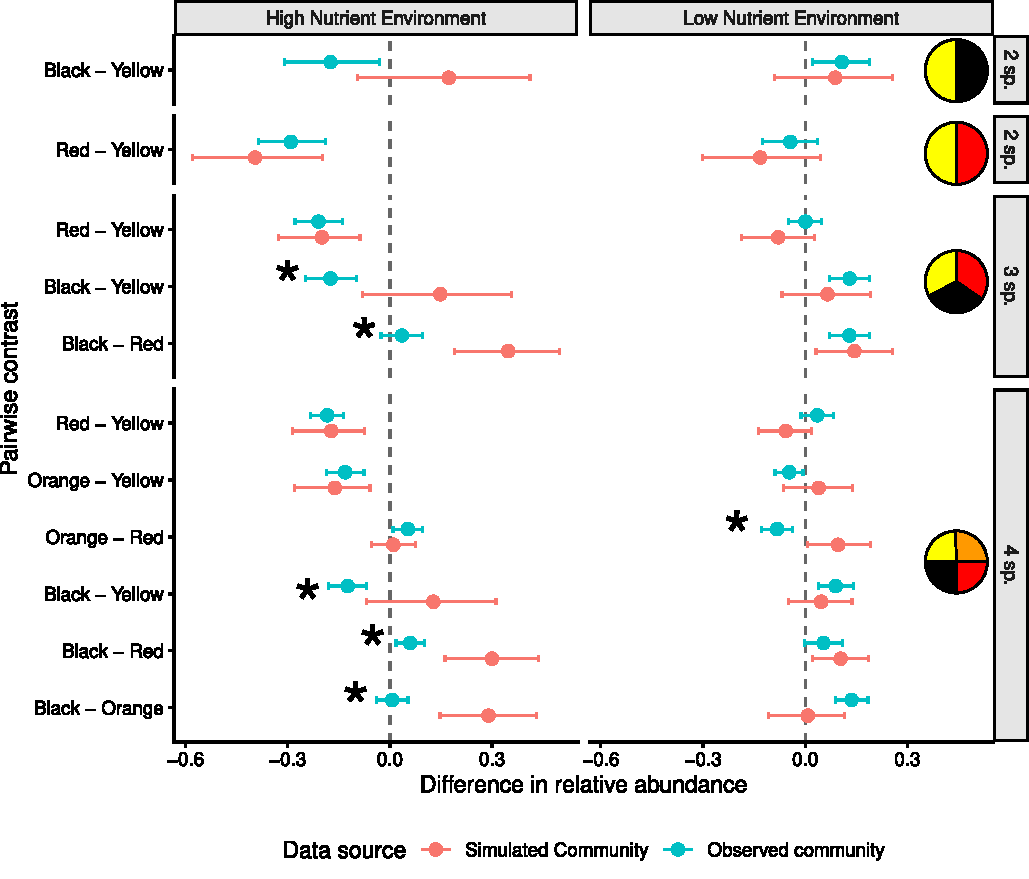
\includegraphics[width=\textwidth, alt={Pairwise contrasts of strain relative abundance estimates across simulated and observed multi-strain communities}]{NutrientNeutrality/Figures/ContrastSummary.pdf}
    \caption[Pairwise contrasts of strain relative abundance estimates across simulated and observed multi-strain communities]{Pairwise contrasts of strain relative abundance estimates across simulated (red) and observed (blue) multi-strain communities. Points represent posterior mean estimates, while horizontal lines represent 95\% credible intervals. Dashed vertical lines mark zero, indicating no difference in final relative abundance between the two strains in a given contrast. Stars indicate contrasts where the 95\% credible intervals for simulated and observed estimates do not overlap. Overall, deviations from neutrality were larger in high-nutrient environments (left) than in low-nutrient environments (right). In three- and four-species communities, observed black-strain relative abundance was lower than expected from simulations parameterized using single-species vital rates.}
    \label{fig:Contrasts}
  \end{center}
\end{figure}